\newpage
\fancyhead[C]{Thomas Turner}
\section{Custom Hardware} \label{section:Custom Hardware}
\subsection{Introduction}\label{sub_section:tgt_custom_hardware_intro}
Due to the specific operating environment, custom hardware is required. This is because the device cannot safely carry out emergency landing procedures when a fault is detected due to the difficulty of retrieval. Furthermore, any crashes can damage the onboard imaging sensors. Lastly, there is significant opportunity cost of delaying mapping as the equipment and manpower involved in demining would be ineffective until retrieval and repair or replacement of the device. 
\paragraph{When to use custom components}
\gls{COTS} options should always be considered before any custom part due to the significant design and testing costs associated with custom parts. Furthermore, \gls{COTS} options will often have shorter lead times and will benefit from sourcing at greater scales. However, when there are specific design requirements not met in the current market custom components need to be used.
\paragraph{Objectives}
All hardware should be easy and quick to debug, it should support redundancy and it should be as modular as possible. Furthermore, they should also line up with our sustainability and inclusion objectives by ensuring all components are \gls{RoHS} compliant and, where applicable, should support those with disabilities. I will design core components demonstrating the design principles explored however, not all hardware components are considered and there is significant room for future work.

\begin{figure}[htbp]
 % Row 2: Legend + GNSS Gerber and Render
  \centering
  \begin{subfigure}[b]{0.48\textwidth}
    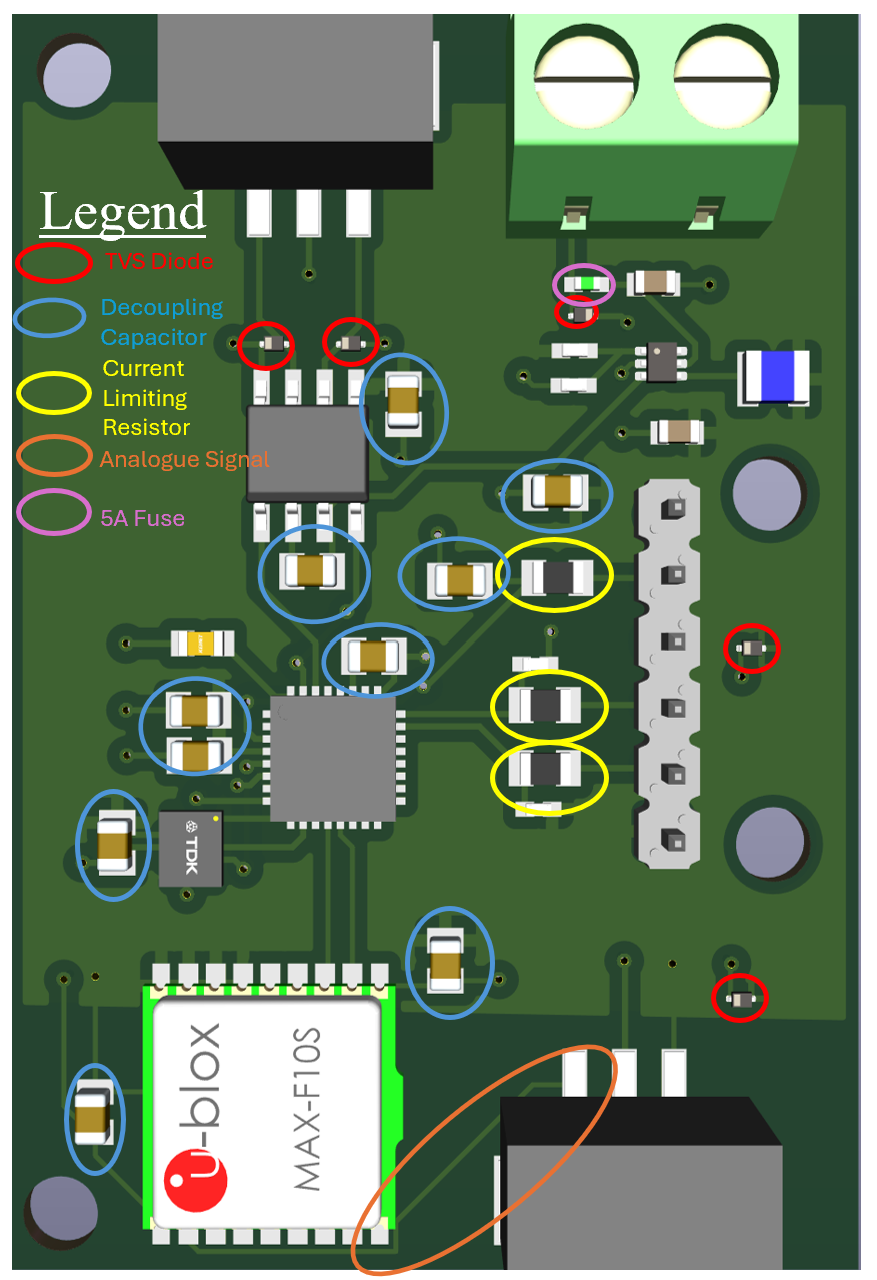
\includegraphics[width=\textwidth]{figs/Thomas/Custom Hardware/GPS render.png}
    \caption{GNSS Module Render}
    \label{fig:gnss_render}
  \end{subfigure}
  \hfill
  \begin{subfigure}[b]{0.48\textwidth}
    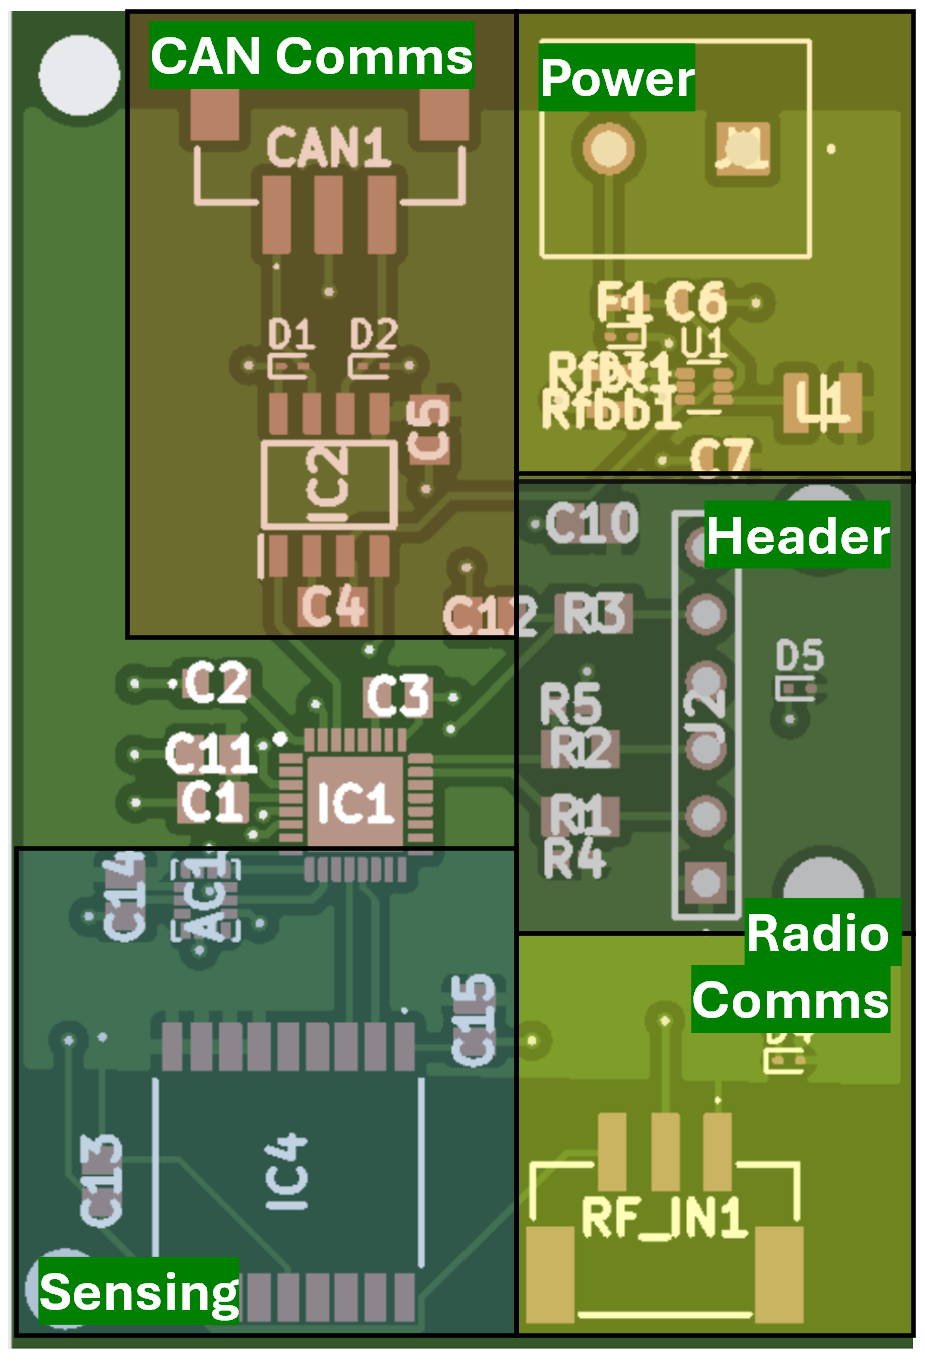
\includegraphics[width=\textwidth]{figs/Thomas/Custom Hardware/GPS gerber.png}
    \caption{GNSS Module Gerber}
    \label{fig:gnss_gerber}
  \end{subfigure}

  
  \begin{subfigure}[b]{0.48\textwidth}
    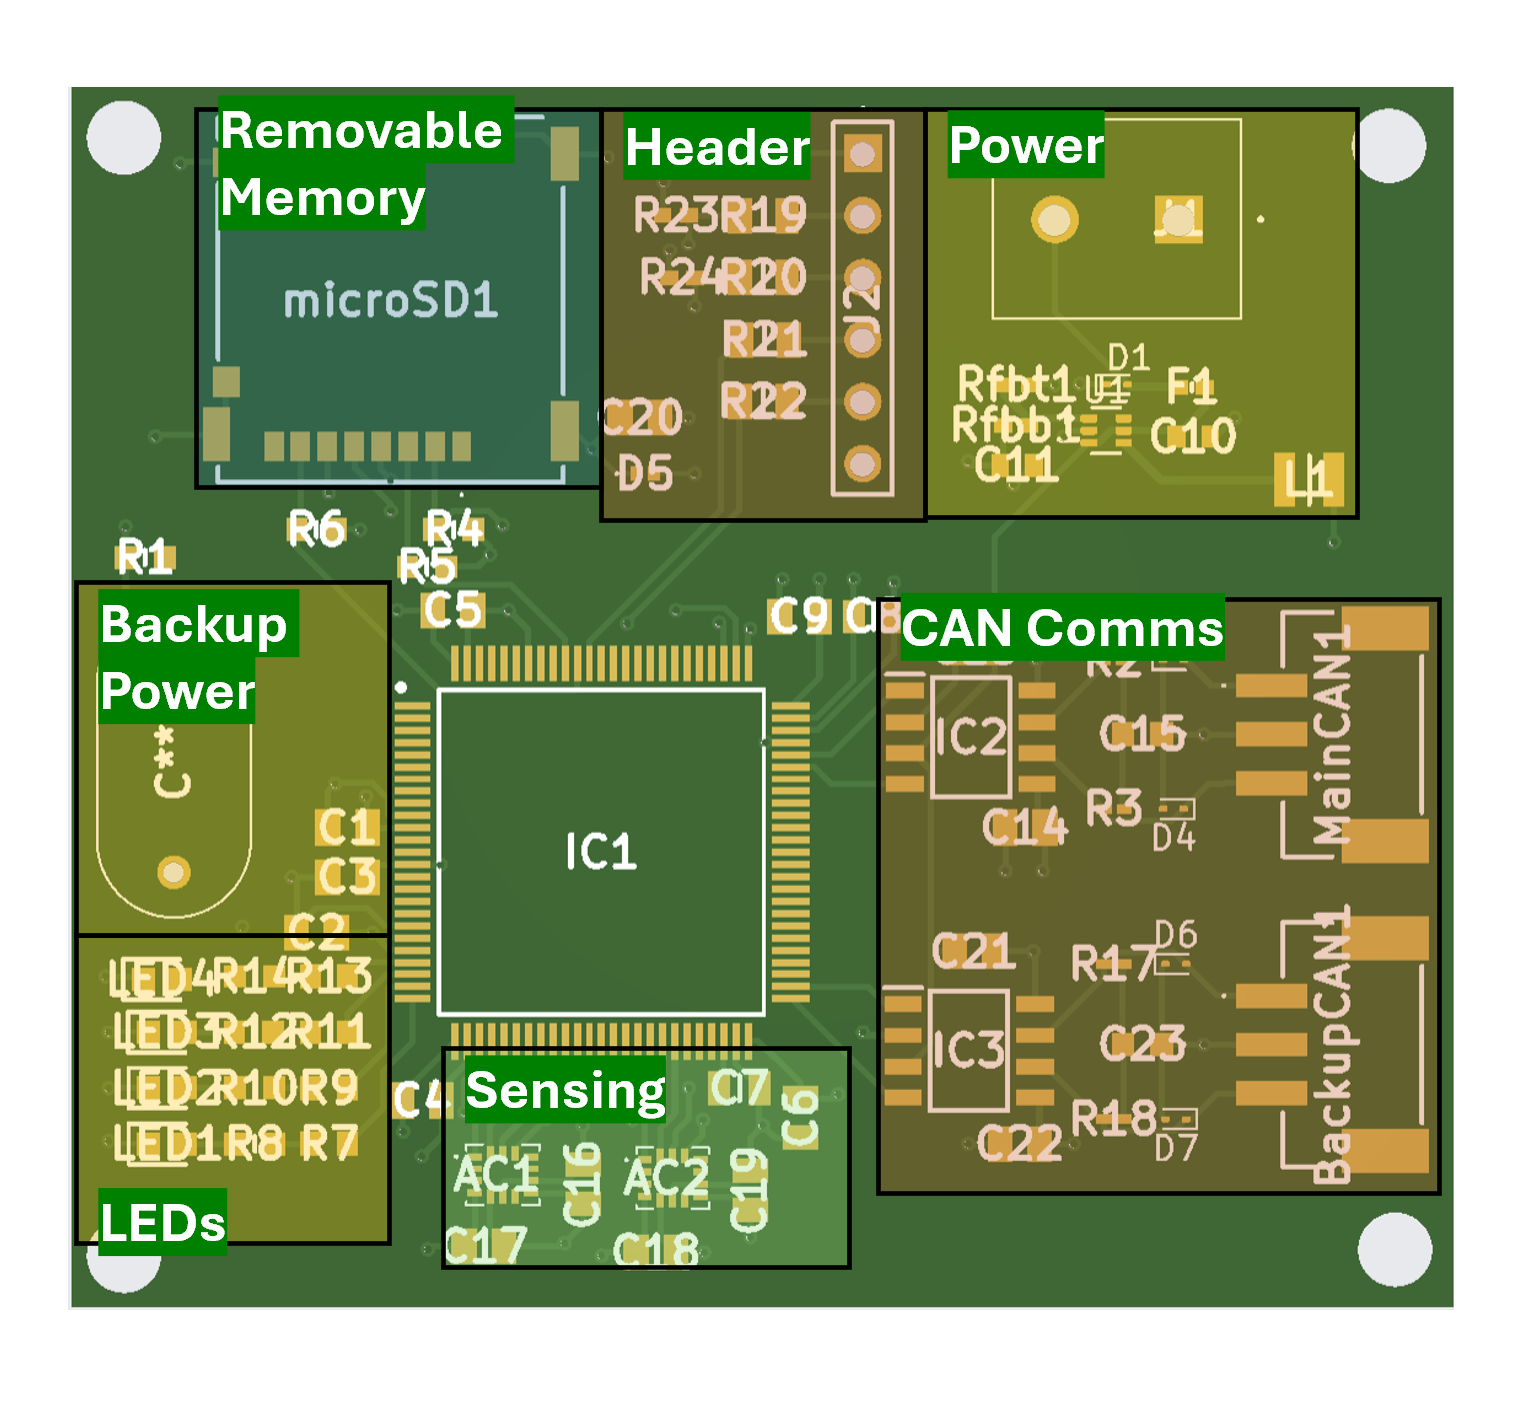
\includegraphics[width=\textwidth]{figs/Thomas/Custom Hardware/FC gerber.png}
    \caption{Custom Flight Controller Gerber}
    \label{fig:fc_gerber}
  \end{subfigure}
  \hfill
  \begin{subfigure}[b]{0.48\textwidth}
    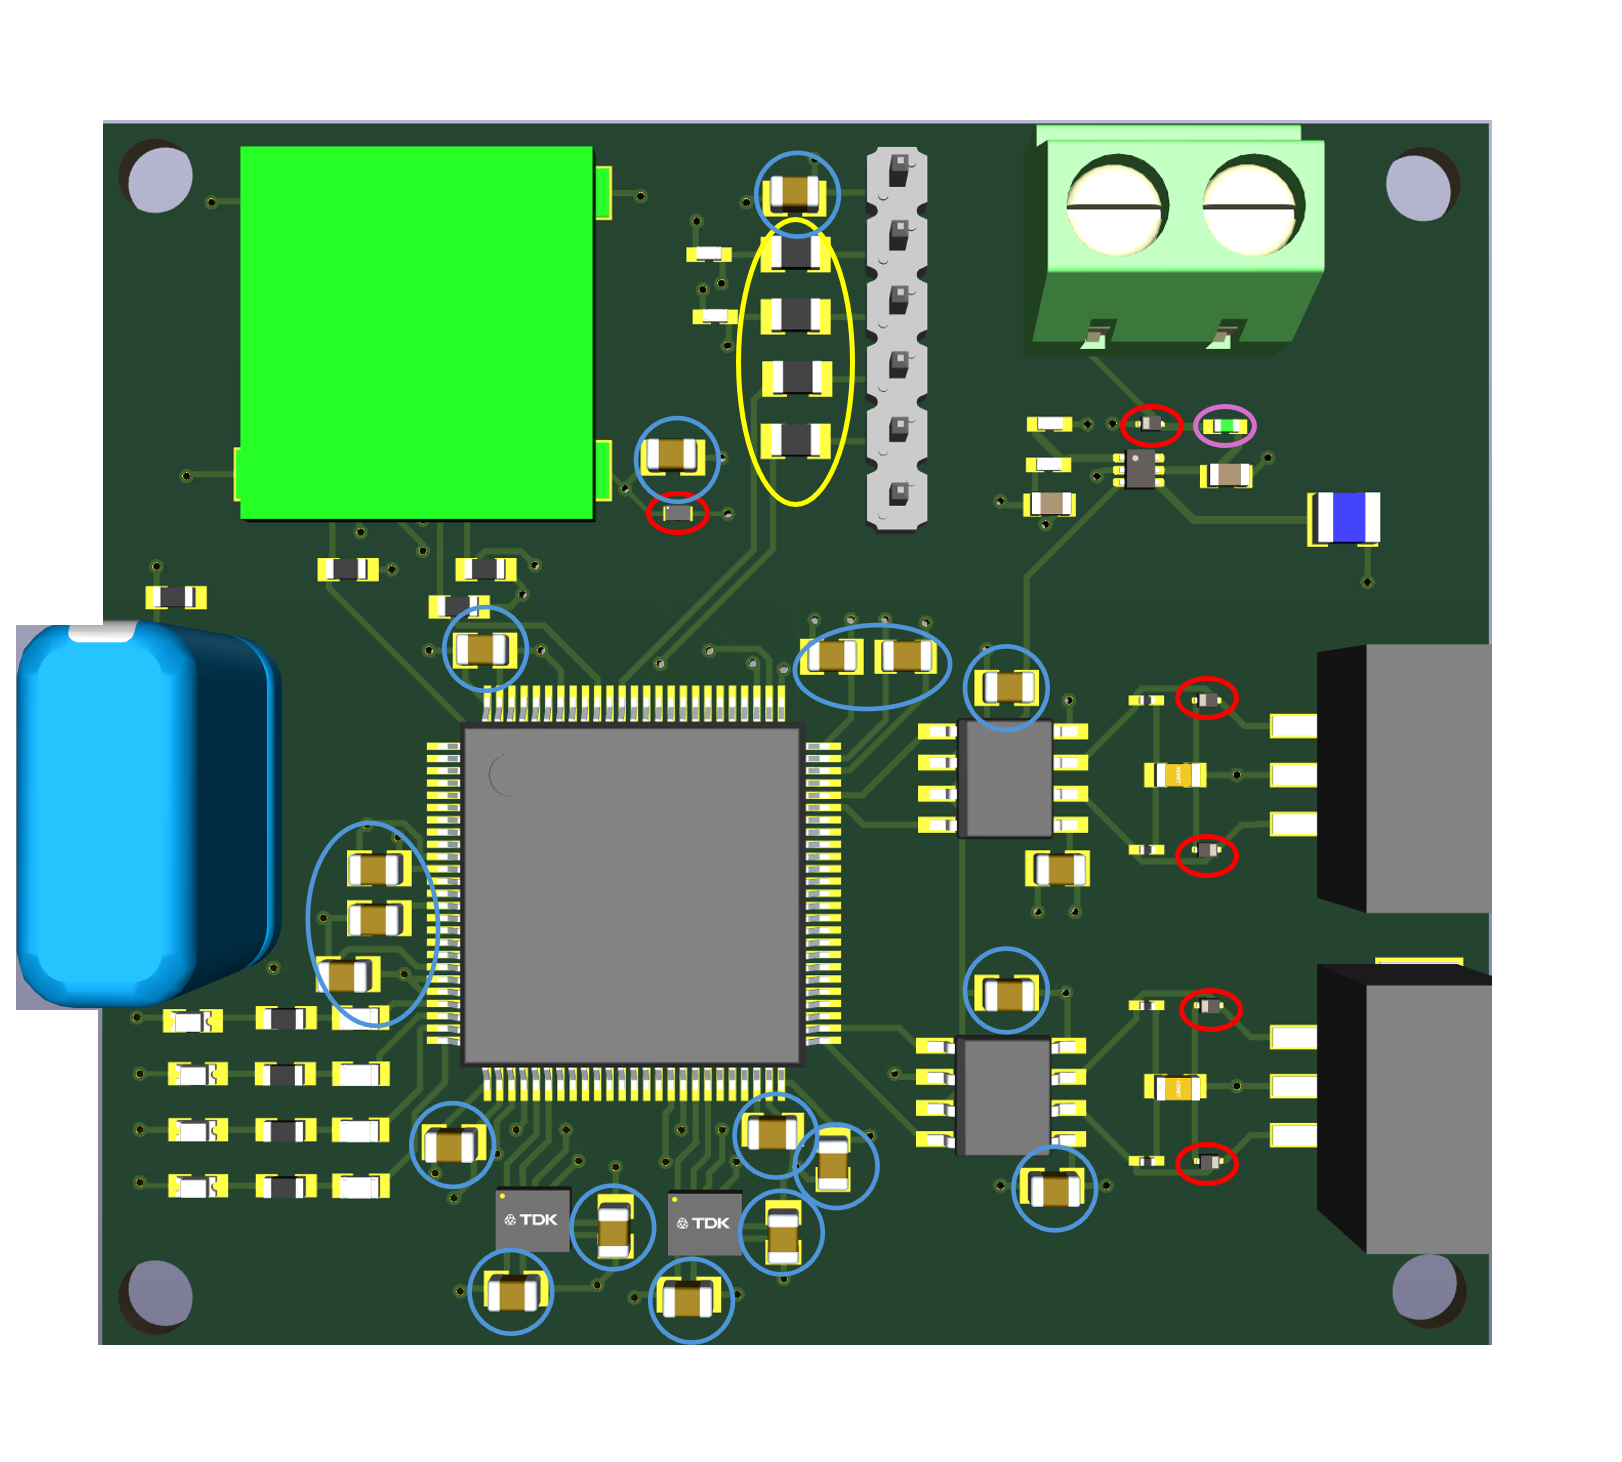
\includegraphics[width=\textwidth]{figs/Thomas/Custom Hardware/FC render.png}
    \caption{Custom Flight Controller Render}
    \label{fig:fc_render}
  \end{subfigure}

  \vspace{1em} % space between rows
  \caption{Custom Hardware Boards: Flight Controller and GNSS Module with Legend}
  \label{fig:custom_hardware_overview}
\end{figure}

\subsection{Design Considerations}

\subsubsection{Trace Lengths}
\paragraph{Signal Integrity and Timing}
All traces have propagation delay that increases linearly with length \cite{REF} meaning that the longer the trace, the longer the delay. Furthermore, noise increases due to impurities and crosstalk. Therefore, traces should be kept as short as possible. This means that large footprint devices are placed at the edges and the \gls{MCU} is placed centrally.
\paragraph{Length Matching}
In synchronous communication methods the clock signal must be in sync with the data transmission. This means that the lines should be as similar in length as possible so that they arrive at the same delay. The faster the communication rate the stricter this must become as the clock signal frequency is increased \cite{REF}.
\paragraph{Effect of vias}
Vias allow for the transference of signals between planes which is necessary for routing signals. However, they should be avoided as they introduce extra impedance, noise and delay. Furthermore, for synchronous high speed signals they should be included in trace length considerations as the line with fewer vias should be tuned to have a longer length to achieve the same delay.

\subsubsection{Protection}
\paragraph{\gls{ESD}}
\gls{ESD} occurs when there is a significant static charge built up in a ground operator or contacting surface that is then shorted in contact with the board. As electro-static voltages can be xxV \cite{REF} this can cause significant damage to devices due to transient current spikes.
\paragraph{Touch Protection Devices}
In order to protect against \gls{ESD} the circuit must provide a low resistance pathway to the ground. This can be using \gls{TVS} diodes that above certain voltages act like a wire that diverts the current flow. They can also be mitigated using voltage dependent resistors that increase resistance with voltage, preventing current spikes. In my designs I make use of bidirectional \gls{TVS} diodes due to their price and simplicity. 
\paragraph{Over current protection}
Fuses and resistors are the best way to protect a device against short circuits. Series resistors mitigate the peak current therefore, for serial debugging I ensured that all connections direct to the \gls{MCU} have series resistors in case of accidental short circuits by the user. However, fuses are the best way to protect against short circuits. This is because, series resistors dissipate too much power to be efficient in power transfer lines, therefore 5A fuses are used in the power lines of both modules. 
\paragraph{Placement}
Protections should be as close to possible sources so the least number of components and wires get damaged in failure. Therefore, all \gls{TVS} diodes are placed near touched areas or interfaces, series resistors are placed as close as possible to prevent wire transients and fuses are placed before the power is connected to the power and ground planes.

\subsubsection{Component Placement}
\paragraph{Utility Regions}
Components with similar functionalities should be restricted to specific regions, this is because it reduces trace length, prevents interference between high and low frequency signals and makes thermal management easier. These regions for the custom designed hardware can be seen in\ref{fig:custom_hardware_overview}.
\paragraph{Thermal Considerations}
Heat dissipating elements, typically diodes and resistors, can cause damage to electronic component, therefore, heat sinks or controlled airflows are sometimes required. This consideration is why on my devices Buck Converters of above 90\% are used instead of the less efficient \gls{LDO} which would have an efficiency of 66\% when converting from 5V to 3.3V. This, in addition to the low power draws of all other components, means that no explicit thermal management is needed.

\subsubsection{Trace Widths and Spacing}
\paragraph{Impedance Control}
The impedance of a trace in inverse proportion to its cross sectional area as it acts like a wire \cite{a source}. Since the trace thickness standard as one ounce per square foot \cite{source} it is the cheapest to manufacture with and is used. Therefore, to control the impedance of a trace the width must be calibrated. \textbf{a nice table showing the widths and current capacities and specific operations}
\paragraph{Crosstalk}
When traces are too close too each other they can induce signals in each other \cite{REF}. However, since all the signals are digital or physically isolated on the board this is not a major concern but I did ensure that all traces are at least 1.5 trace widths separated as a form of best practice. Furthermore, the Radio Frequency input for the \gls{GNSS} module is kept away from all other components and the ground and voltage planes as shown in \ref{fig:gnss_render}).

\subsubsection{Layers}
\paragraph{Two Layers}
The simplest and most cost effective option in \gls{PCB} design is two copper layers separated by a dielectric \cite{REF}. By using a copper filled regions you can create a ground plane and a power plane that effectively distribute charge and maintain voltage integrity. The simplicity of the \gls{GNSS} module means that two layers is the best option. This comes at the cost of more difficult component placement and a slightly less stable power and ground plane. To mitigate the instability, distributed ceramic capacitors between the planes that filter high frequency noise in voltage levels, maintaining integrity. These capacitors are best placed next to sensors and processers to ensure stable, low noise readings.
\paragraph{Four or More Layers}
When circuits become more complex, a purpose ground and power plane in between the top and bottom plane can allow for greater packing density of components. They also make the planes more stable as all the path impedances are very low. This means that for complex designs with many sensors, like the flight controller module, four layer \gls{PCB}s are the best option. Furthermore, if the complexity of the design is greater you can add further ground and power planes for analogue signals, high frequency signals or for regular signals to support greater component density.

\subsection{Debugging}
\paragraph{Technical Debugging}
There easy to use male pin headers in both designs shown in \ref{fig:custom_hardware_overview} so that a \gls{SWD} debugger can be connected, furthermore, for signalling debugging the detachable ports for the \gls{CAN} bus mean a debugging computer can simply connect. This is so technically skilled operators can inspect system level signals and specific board operations.
\paragraph{Field Debugging}
The use of technical debugging experts should always be avoided if possible to reduce capital expenditure and delay. Therefore the custom flight controller has a simple 4 \gls{LED} array for basic error codes that can isolate the problem so it can be fixed or so that only a specific, replaceable component, can be sent for repair and switched out with a backup. These codes are shown in \ref{tab:error_codes} where the colours are the \gls{LED}s and the x denotes blinking, the null state is a solid green \gls{LED} only.  The inclusion of the green LED has three key purposes: firstly, it blinks to denote between modules, secondly it gives clear visualisation that no tests have failed and lastly it ensures the codes are red in the right order no matter the orientation. It is also a different brightness to the red \gls{LED}s allowing for use by colour-blind operators in line with the inclusion objectives of the project.
\begin{table}
\centering
\begin{tabular}{|l|c|l|c|l|c|l|c|}
\hline
\textbf{Failure} & \textbf{Code} & \textbf{Failure} & \textbf{Code}& \textbf{Failure} & \textbf{Code} & \textbf{Failure} & \textbf{Code} \\
\hline
CAN 1 & \drawcode{white}{red}{red}{red} & CAN 2 & \drawcode{blinkgreen}{red}{red}{red} &
GNSS 1 & \drawcode{white}{red}{red}{white} & GNSS 2 & \drawcode{blinkgreen}{red}{red}{white}\\

Flight Controller & \drawcode{white}{red}{white}{white} & BMS & \drawcode{blinkgreen}{red}{white}{white} &
Collision 1 & \drawcode{white}{white}{red}{white} & Collision 2 & \drawcode{blinkgreen}{white}{red}{white}\\

ESC 1 & \drawcode{white}{blinkred}{blinkred}{blinkred} & ESC 2 & \drawcode{white}{red}{blinkred}{blinkred} &
ESC 3 & \drawcode{white}{red}{red}{blinkred} & ESC 4 & \drawcode{white}{red}{blinkred}{red}\\

Altimetry 1 & \drawcode{white}{white}{white}{red} & Altimetry 2 & \drawcode{blinkgreen}{white}{white}{red} &
LoRa & \drawcode{white}{white}{red}{red} & Unknown & \drawcode{blinkgreen}{blinkred}{blinkred}{blinkred}\\
\hline
\end{tabular}
\caption{Flight Controller LED Error Codes}
\label{tab:error_codes}
\end{table}
\paragraph{Post Failure Analysis}
If there is a crash that causes significant damage, and due to the volatile nature of \gls{RAM} memory, some failures cannot be detected directly with the device. Therefore, the flight controller has a removable microSD card to record flight data. In addition, the backup power supply, as seen in \ref{fig:custom_hardware_overview}, provides enough power that even in complete failure it can write the final few error messages. Therefore, this can be retrieved, downloaded and sent for analysis quickly to find the source of failure.
\subsection{Custom Components}\label{sub_sub_section:tgt_custom_components}

\subsubsection{Component Selection}\label{sub_sub_section:tgt_component_selection}


\paragraph{\gls{IMU}}
While the BMI323 is cheaper it has higher noise characteristics than the the ICM-42688-P, therefore the latter was selected for use on all boards due to its low price point and high performance. The use of the same \gls{IMU} over all modules should be maintained if possible so that the control characteristics are unchanged across devices and lower costs due to higher order quantities.
\paragraph{\gls{MCU}}
For the flight controller the STM32H743VGT6 is the best option given its \gls{RAM}, price point and support of dual \gls{CAN} buses. However, for the less computationally intense operations required for the \gls{GNSS} module the smaller footprint (due to the lower number of pins) and lower priced MSPM0G3506SRHBR is a better option.
\paragraph{\gls{GNSS} Module}
Exact positions for where the images were taken to cm precision is required as discussed in Section \ref{GPR_design}, this is possible using a \gls{RTK} setup with a base station sending out correction vectors over LoRA getting within cm accuracy\cite{RTK_LORA}. Furthermore, in the case of the loss of all \gls{GNSS} signal built in dead reckoning, allowing \gls{RTS}, is also a desirable feature. Therefore, the LG69T-AP is selected. However, when not executing imaging tasks, this precision is not needed and the modules are more expensive than the \gls{GNSS} modules without these features. Therefore, for the redundant device the MAX-F10S-00B was selected, and is shown in \ref{fig:custom_hardware_overview}, due to the significantly better documentation available and similar price points when compared to the LC29HAAMD.

\subsubsection{Power Supply}\label{sub_sub_section:tgt_power_supply}
\begin{table}[htbp]
  \centering
  \begin{tabular}{lrrr}
    \toprule
    \textbf{Component} & \textbf{Flight Controller} & \textbf{Redundant GNSS} & \textbf{Value}\\
    \textbf{} & \textbf{Quantity} & \textbf{Quantity} & \textbf{(mA)}\\ 
    \midrule
    ICM-42688-P\tablefootnote{\url{https://invensense.tdk.com/products/motion-tracking/6-axis/icm-42688-p/}} & 2  & 1 & 0.88\\
    STM32H743VGT6\tablefootnote{\url{https://www.st.com/en/microcontrollers-microprocessors/stm32h743vg.html}} & 1 & 0 & 165\\
    MSPM0G3506SRHBR\tablefootnote{\url{https://www.ti.com/product/MSPM0G3506/part-details/MSPM0G3506SRHBR}} & 0 & 1 & 8\\
    MAX-F10S-00B\tablefootnote{\url{https://www.u-blox.com/en/product/max-f10s-module}} & 0 & 1 & 200\\
    LEDs & 3 & 0 & 20 \\
    Misc & 1 & 1 & 20 \\ 
    \midrule
    \textbf{Total} & \textbf{246.76 mA} & \textbf{228.88 mA} & \textbf{}\\
    \bottomrule
  \end{tabular}
  \caption{Current Draws}
  \label{tab:current-draws}
\end{table}
\paragraph{Main Power Supply}
In both the GNSS module and the flight controller module the same power setup was used, created in Webench Power Designer\footnote{\url{https://webench.ti.com/power-designer/switching-regulator}}. The key decision metrics were efficiency and cost.  Efficiency is of high importance due to the thermal management on the board. The design selected has over 90\% efficiency \ref{fig:power_graphs} throughout the expected operating current window. As shown in the schematic \ref{fig:power_supply_schematic} there is a fuse to protect from short circuits and a \gls{TVS} diode to protect against \gls{ESD} that someone connecting the power might cause. There are also capacitors of 22uF and 4.7uF to provide current during spikes and smooth the power supply current.
\begin{figure}[htbp]
  \centering
  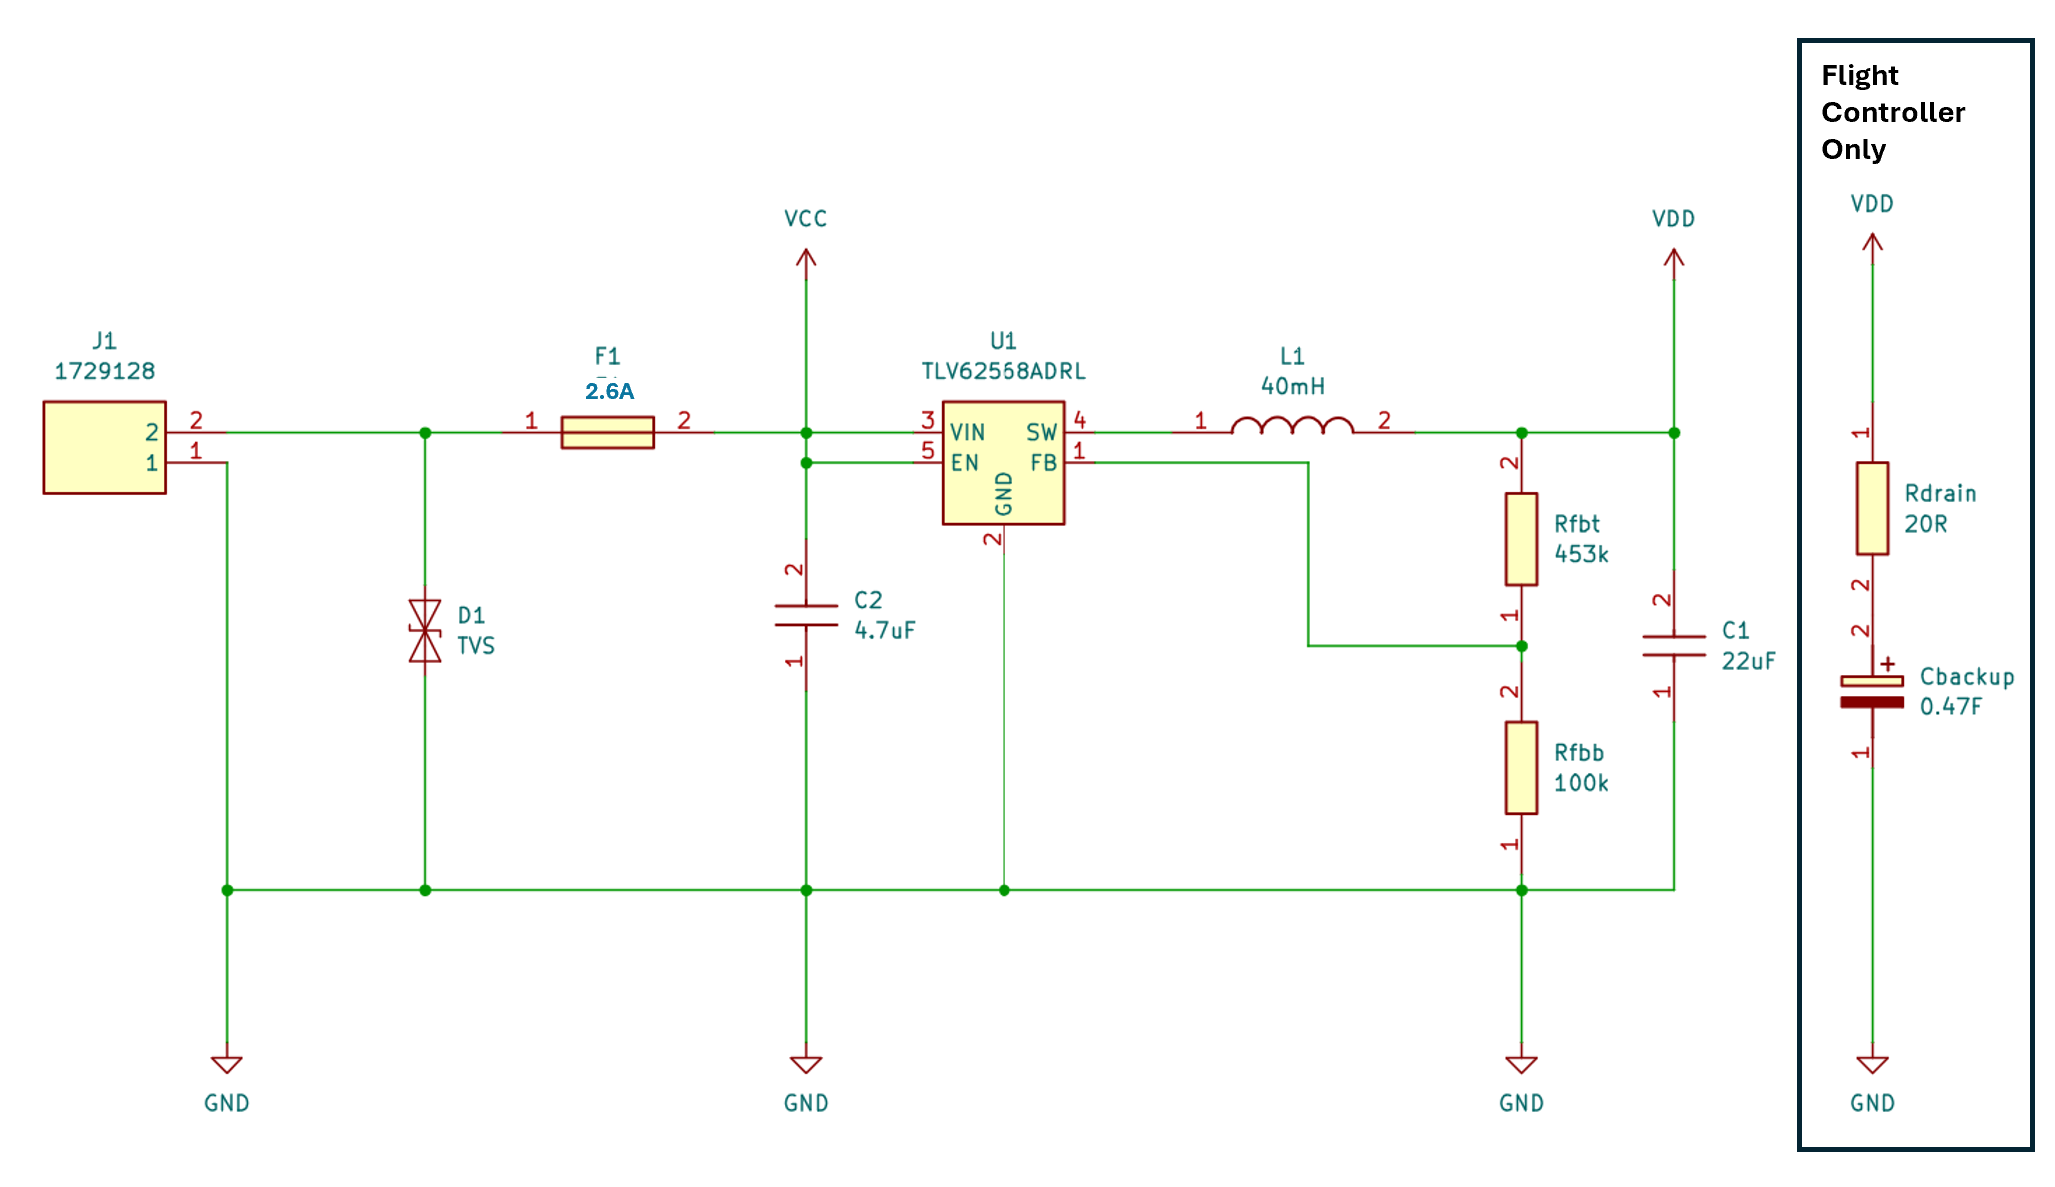
\includegraphics[width=\textwidth]{figs/Thomas/Custom Hardware/Power Supply.png}
  \caption{Power Supply Schematic}
  \label{fig:power_supply_schematic}
\end{figure}



\begin{figure}[htbp]
  \centering
  \begin{subfigure}[b]{0.48\textwidth}
    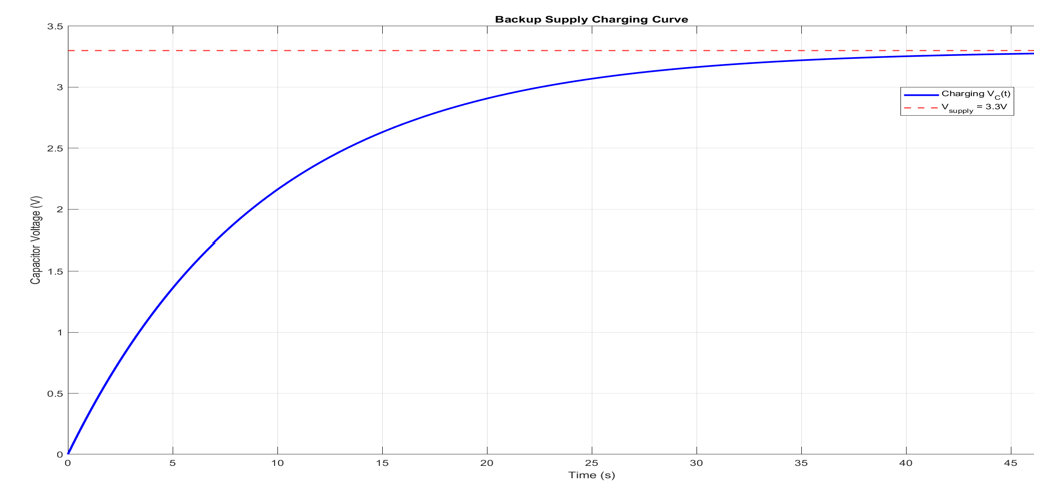
\includegraphics[width=\textwidth]{figs/Thomas/Custom Hardware/charging_curve.png}
    \caption{Backup Power Supply Charging Curve}
    \label{fig:charging_curve}
  \end{subfigure}
  \hfill
  \begin{subfigure}[b]{0.48\textwidth}
    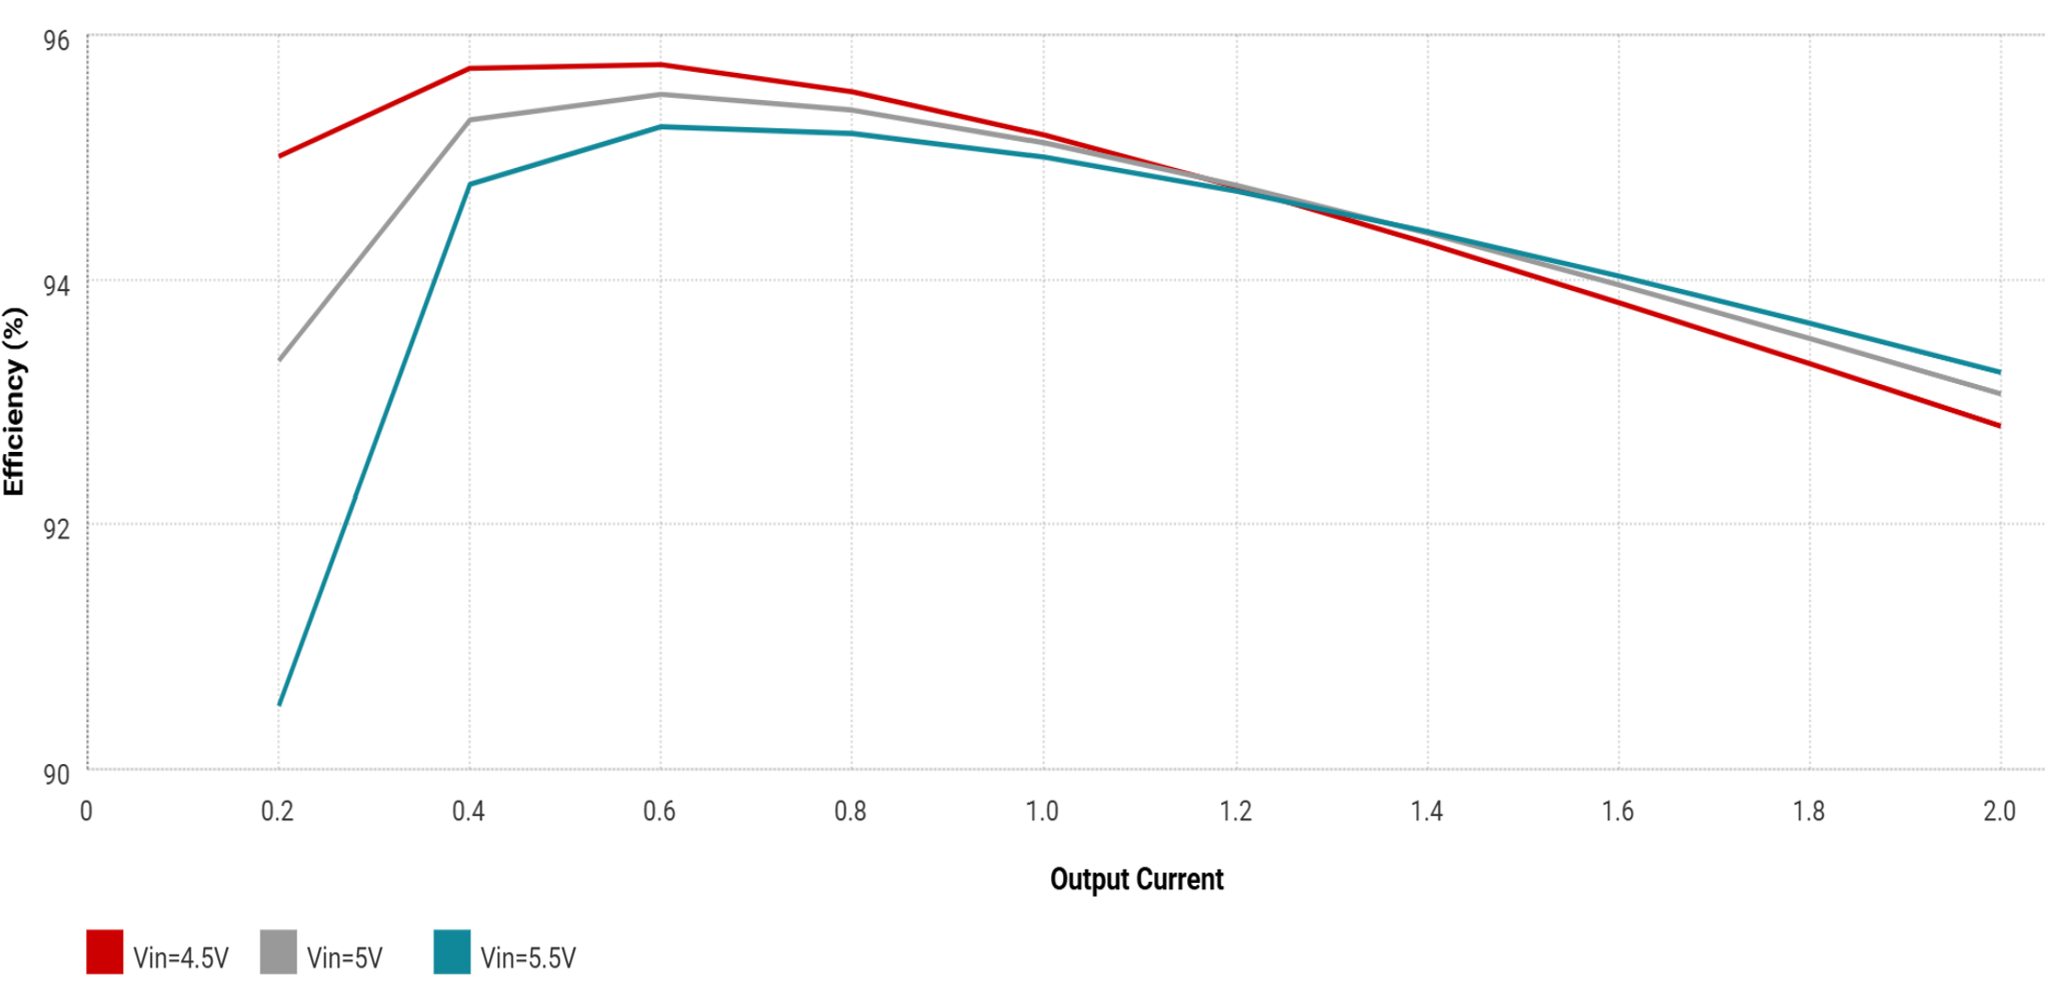
\includegraphics[width=\textwidth]{figs/Thomas/Custom Hardware/Power Module Effciency.png}
    \caption{Power Module Efficiency}
    \label{fig:power_efficiency}
  \end{subfigure}
  \caption{Custom Power Supply}
  \label{fig:power_graphs}
\end{figure}

\paragraph{Backup Power Supply}
The telemetry recordings of the flight controller are vital for crash analysis. However, in cases of sudden electrical failure the data recording will stop before writing the final state vectors and error codes. For example, if before a short circuit the current draw from an \gls{ESC} starts spiking that message needs to be recorded even if a fuse immediately burns shutting down the power supply. Therefore, a supercapacitor in series with a drain resistor is used \ref{fig:power_supply_schematic}. The capacitor selected is rated up to 5.4V at 0.47F\footnote{\url{https://uk.rs-online.com/web/p/supercapacitors/2506967}}. 
\begin{equation}
t = \frac{C \cdot (V_0 - V_{\text{cutoff}})}{I}
\label{eq:discharge_time}
\end{equation}
\begin{equation}
t_{\text{worst-case}} = \frac{0.47 \cdot (3.3 - 2.8)}{1} = 0.235\ \text{seconds}
\label{eq:worst_case_time}
\end{equation}
\begin{equation}
\tau = R \cdot C = 20 \cdot 0.47 = 9.4\ \text{seconds}
\label{eq:charging_time_constant}
\end{equation}
The time before dropout, with the worst case conditions is over 0.2 seconds \ref{eq:worst_case_time}, this will provide sufficient time to record any last messages. Furthermore, the time constant is 9.4s \ref{eq:charging_time_constant} meaning that there are current spikes when turning the device on but it is still charged over 3V within 30 seconds \ref{fig:charging_curve}.

\subsubsection{Comparison to Commercial Options}\label{sub_sub_section:tgt_commercial_options}
\begin{table}[htbp]
  \centering
  \begin{tabular}{|l|r|r|}
    \hline
    \textbf{Category}         & \textbf{Redundant GNSS Cost} & \textbf{Flight Controller Cost}\\ 
    \hline
    Passive Components        & £140.40  & £385.00\\
    Active Components         & £1699.10 & £1865.10\\
    Headers/Connectors        & £179.50  & £278.40\\
    PCB \& Assembly           & £262.14  & £334.04\\
    \hline
    \textbf{Total}            & £2281.14 & £2862.54\\
    \hline
  \end{tabular}
  \caption{Cost of custom component (100 units)}
  \label{tab:aggregated-cost}
\end{table}
The CUAV X7+\footnote{\url{https://store.cuav.net/shop/x7/}} GPS compatible option costs £339.75 and provides the same core functionality as the custom flight controller including dual \gls{CAN} ports. This can be combined with the flight controller compatible with the CUAV C-RTK 9Ps Positioning Module\footnote{\url{https://store.cuav.net/shop/c-rtk-9ps/}} that costs £332.91 for a drone-base station pair and provides \gls{RTK} \gls{GNSS}. This is a significant increase in cost however, it would not require development and may be a superior option in the testing phase. However, for deployment the custom components should be used given the cost implications and that the custom \gls{GNSS} module is fully control capable and the commercial option is not. 
